\section{Автоматизация определения конфигурации обманной системы}

Одной из главных особенностей применения обманных систем является сложность выбора конфигурации \citep{rajan}. Количество, расположение и конфигурацию ловушек необходимо выбирать так, чтобы их применение было максимально эффективным. Для автоматизации данного процесса необходимо свести топологическую и функциональную модели защищаемой сети к некоторой математической модели. Она позволит применять существующие методы для решения поставленной задачи.

\subsection{Математическая модель защищаемой сети}

Предлагается исходить из следующих основных предположений:
\begin{itemize}
	\item для защищаемой сети актуальны атаки направленного типа;
	\item в сети выделяются две особые группы узлов: узлы, обрабатывающие критическую информацию, и узлы, непосредственно доступные для воздействия потенциального нарушителя;
	\item сеть обладает связностью, то есть из любой ее точки можно передать данные в любую другую точку за конечное число шагов;
	\item направленная атака представляет собой последовательность промежуточных (частных) атак, первая из которых имеет своей целью один из доступных нарушителю до начала атаки узлов, а последняя – один из узлов, работающих с критической информацией;
	\item система защиты информации не имеет достоверных сведений о начале направленной атаки, динамике ее развития, точном списке целей злоумышленника;
	\item нарушитель в начале направленной атаки не имеет достоверных сведений о структуре сети, однако может полностью или частично восстанавливать ее в ходе своих действий.
\end{itemize}

Система защиты должна быть спроектирована таким образом, чтобы вероятность контакта нарушителя с элементами обманной системы была максимально возможной.

Пусть $V$ — множество всех сетевых узлов, включающее как реальные, так и ложные цели. В соответствии с принятыми предположениями целью злоумышленника в ходе реализации направленной атаки является получение доступа к данным, хранящимся на определенных сетевых узлах в критических областях сети $V_{cr} \subset V$. Должен учитываться тот факт, что не все узлы одинаково доступны злоумышленнику и что на разных этапах атаки он может атаковать различные подмножества. Пусть $V_{avail,i} \subset V, i \in [0, k]$ - множество узлов, доступных нарушителю для атаки на шаге с номером $i$. Множество $V_{avail,0}$ является множеством потенциальных точек входа злоумышленника в сеть.

Неоднородность сети, вследствие которой множества $V_{avail,0}, ... , V_{avail,k}$ вообще говоря не совпадают между собой, обусловлена принимаемыми в сети мерами разграничения доступа, которые могут быть реализованы, например, в виде правил межсетевого экрана. Обычно правила разграничения сетевого доступа задаются при помощи дискреционной модели. В этом случае каждому узлу сети $v \in V$ можно поставить в соответствие список доступа $A_v = \{ w \in V | w \sim v \}$, где запись $w \sim v$ означает возможность прямой передачи данных между узлами $v$ и $w$.
 
Рассмотрим бинарное отношение $T$, заданное на множестве узлов сети: $T: V \times V \rightarrow \{0, 1\}$ по следующему правилу:
\begin{equation}
\label{eq:bin_network}
T(v_1, v_2) = 
	\begin{cases} 
		1,  & A_{v_1} = A_{v_2} \\
		0,  & A_{v_1} \neq A_{v_2} 
	\end{cases}
\end{equation}

Очевидно, отношение (\ref{eq:bin_network}) является отношением эквивалентности на множестве сетевых узлов. Классы эквивалентности, порожденные им (\ref{eq:netw_split}), обладают следующими свойствами: 

\begin{itemize}
	\item все узлы, входящие в один и тот же класс, одинаково доступны для атаки из всех точек сети;
	\item захват контроля над любым узлом в пределах одного класса дает возможность атаковать одни и те же цели;
	\item между любыми двумя узлами одного класса возможен прямой обмен данными.
\end{itemize}

\begin{equation}
\label{eq:netw_split}
V = V_1 \cup V_2 \cup ... \cup V_n
\end{equation}

На практике такие классы соответствуют областям сети с одинаковой политикой доступа. В случае использования межсетевого экрана в качестве средства разграничения доступа описанные выше классы эквивалентности принято называть зонами межсетевого экрана.

Поскольку направленная атака описывается последовательностью атакуемых узлов, то ее можно однозначно задать с помощью последовательности $\sigma = V_{f_1}, V_{f_2}, ... , V_{f_k}$ зон, через которые нарушитель проходит в рамках атаки.

Взаимную доступность сетевых узлов, находящихся в разных зонах, удобно представлять в виде графа $G = (V, E)$, построенного по следующим правилам:

\begin{itemize}
	\item каждая вершина графа соответствует одной из зон межсетевого экрана;
	\item ребро графа проводится между двумя вершинами, если существует возможность прямой передачи данных между узлами в соответствующих зонах.
\end{itemize}

Обычно, если передача данных возможна в одном направлении, то она возможна и в обратном. Поэтому граф полагается ненаправленным.

Итак, поведение нарушителя в ходе направленной атаки может быть представлено в виде маршрута $\sigma$ в графе $G$. Этим маршрутом определяется порядок прохождения нарушителя через зоны межсетевого экрана. В каждой зоне межсетевого экрана, наряду с реальными, могут размещаться и ложные цели, входящие в состав обманной системы. Нарушитель не может с определенностью утверждать для каждого узла сети, является ли этот узел ложной целью или нет. Это приводит к тому, что при прохождении каждой из зон межсетевого экрана нарушитель может с некоторой вероятностью $P_{honey}$ совершить атаку на элемент ОбС.

Рассмотрим случай, когда все узлы одной зоны имеют одинаковую конфигурацию. Вероятность проведения атаки на элемент ОбС при прохождении зоны $V_{f_i}$ составляет $P_{honey} = l_i / s_i$, где $l_i, s_i$ - количество ложных целей и общее количество узлов в зоне $V_{f_i}$.

Рассмотрим некоторую направленную атаку, представимую в виде маршрута $\sigma = V_{f_1}, V_{f_2}, ... , V_{f_k}$. Вероятность того, что при прохождении некоторой зоны  контакт злоумышленника с ОбС будет отсутствовать составляет $ 1 - l_i / s_i$. Таким образом, вероятность того, что злоумышленник в результате проведения атаки  не попадет на элементы обманной системы составляет:

\begin{equation}
P_{victim} = \prod_{i=1}^k (1 - \frac{l_i}{s_i})
\end{equation}

Соответственно вероятность того, что злоумышленник в результате проведения атаки осуществит контакт с элементом обманной системы составляет:

\begin{equation}
\label{eq:p_honey}
P_{honey} = 1 - \prod_{i=1}^k (1 - \frac{l_i}{s_i})
\end{equation}

Каждый элемент произведения (\ref{eq:p_honey}) представляет собой вероятность контакта нарушителя и ОбС на одном из шагов направленной атаки. Заменим неориентированный граф $G$ на взвешенный ориентированный, проведя дуги в обоих направлениях между всеми инцидентными вершинами исходного графа . Каждой дуге, входящей в вершину $v$, соответствующей некоторой зоне $V_{f_i}$, поставим в соответствие число $w = 1 - l_i / s_i$, равное вероятности прохождения нарушителем области сети  без его обнаружения.

В рамках заданной математической модели задача о нахождении количества, расположения и конфигурации ловушек сводится к нахождению такого распределения элементов обманной сети по вершинам графа $G$, при котором максимизируется минимально возможная вероятность контакта злоумышленника с элементами обманной системы при проведении направленной атаки. Минимально возможная вероятность рассчитывается:

\begin{equation}
\label{eq:p_honey_min}
P_{honey, min} = \min_{\sigma \in S} P_{honey, \sigma} 
\end{equation}
где $S$ - множество всех возможных направленных атак на критические области $V_{cr}$.

Описанная модель работает в условиях, когда все узлы одной зоны имеют одинаковую конфигурацию. Данная модель расширяется до модели с поддержкой различных конфигураций следующим образом: каждую зону можно разбить на множества узлов с одинаковой конфигурацией

\begin{equation}
\label{eq:multi_conf}
V_{i} = V_i^{c_1} \cup V_i^{c_2} \cup ... \cup V_i^{c_m}, c_j \in C
\end{equation}
где $C$ - множество всех различных конфигураций в защищаемой сети.

Таким образом, всякой последовательности сетевых узлов можно поставить в соответствие последовательность множеств $V_i^{c_j}$. От графа $G$ можно перейти к графу $G'$, в котором вершинами являются множества узлов , при этом множество ребер преобразуется следующим образом:

\begin{itemize}
	\item в множестве $\{V_i^{c_{j_1}},..., V_i^{c_{j_k}}\}, V_i^{c_{j_l}} \neq \emptyset$, которое является разбиением типа (\ref{eq:multi_conf}) узла, соответствующему зоне $V_i$, присутствуют связи между каждой парой элементов;
	\item в случае наличия в графе $G$ ребра между узлами, соответствующими зонам $V_i$ и $V_j$, в графе $G'$ будут добавлены ребра для каждого множества из разбиений $V_i$ и $V_j$ типа (\ref{eq:multi_conf});
	\item веса ребер рассчитываются аналогично графу $G$.
\end{itemize}

Таким образом мы получили математическую модель защищаемой сети, поддерживающую наличие различных конфигураций.

\subsection{Решение оптимизационной задачи распределения ловушек}

Задача о нахождении количества, расположения и конфигурации ловушек свелась к оптимизационной задачи с целевой функцией задаваемой формулой (\ref{eq:p_honey_min}).

Существует большое количество способов решения оптимизационной задачи при помощи эвристических методов. В данной работе будет использоваться метод решения при помощи генетических алгоритмов.

Генетический алгоритм при помощи последовательных преобразований, схожих с процессами в модели биологической эволюции, над множеством промежуточных решений осуществляет поиск экстремумов заданной целевой функции. Для решения полученной оптимизационной задачи будет использоваться алгоритм \textit{NSGAII}. Данный алгоритм ориентирован на решение мультикритериальных задач, однако его концепция подходит и для решения однокритериальной задачи. \textit{NSGAII} при помощи специальных операторов селекции и дополнительного шага вытеснения доминирующих решений позволяет поддерживать равномерную с точки зрения целевой функции плотность популяции, обеспечивая таким образом более равномерную сходимость \citep{NSGA2002}.

Для применения выбранной реализации генетического алгоритма необходимо решить следующие подзадачи:
\begin{itemize}
	\item определить способ кодирования решения;
	\item сформировать целевую функцию и определить способ ее вычисления по заданному решению;
	\item выбрать операторы скрещивания и мутации.
\end{itemize}

\subsubsection{Кодирование решения}\hspace*{\fill} \\

По выработанной математической модели фактическое распределение элементов обманной системы определяется количеством ловушек присутствующих в каждой зоне $V_i, i=1..n$ из разбиения (\ref{eq:netw_split}). Таким образом распределению ловушек можно поставить в соответствие целочисленный вектор-хромосому (\ref{eq:solution}).

\begin{equation}
\label{eq:solution}
D = (h_1,h_2,...,h_n) 
\end{equation}
\begin{explanation}
где & $n$ & количество зон из разбиения (\ref{eq:netw_split});\\
	& $h_i$ & количество ловушек в зоне $V_i$.
\end{explanation}


\subsubsection{Целевая функция}\hspace*{\fill} \\

Полученная целевая функция (\ref{eq:p_honey_min}) определяет минимально возможную вероятность контакта злоумышленника с элементами обманной системы, однако в распределении ловушек присутствует еще такой важный фактор как количество задействованных агентов. Необходимо по возможности сокращать количество ловушек в системе для уменьшения потребления ресурсов с сохранением максимально возможного значения $P_{honey, min}$. Данный фактор можно выделить как отдельный критерий, однако технологии мультикритериальной оптимизации нацелены на получение множества компромиссных с точки зрения заданных критериев решений. В нашем случае ситуация обратная: в первую очередь необходимо максимизировать значение вероятности и только среди множества решений с максимально возможным значением вероятности выбирать решение с минимальным количеством задействованных ловушек. Для решения описанной проблемы необходимо объединить оба критерия в одну скалярную функцию.

Значение (\ref{eq:p_honey_min}) лежит в диапазоне $[0, 1]$, при этом данную вероятность можно рассматривать с некоторой точностью до $k$ знаков после запятой. В рамках данной модели достаточно принять $k$ равное $5$, так как общее количество узлов $s_i$ в некоторой зоне $V_j$ на практике практически всегда меньше 10000, поэтому изменение в распределении ловушек  даже в случае столь крупных зон обязательно затронет более старшие знаки.

Таким образом целевая функция будет иметь вид (\ref{eq:fitness}).

\begin{equation}
\label{eq:fitness}
f(D) = (1 - \min_{\sigma \in S} P_{honey, \sigma}) + 10^{-5} \sum_{i=1}^n h_i
\end{equation}
\begin{explanation}
где & $D$ & распределение ловушек (\ref{eq:solution}); \\
	& $S$ & множество всех возможных направленных атак на критические области $V_{cr}$. \\
\end{explanation}

Значение $\min_{\sigma \in S} P_{honey, \sigma}$ было инвертировано в формуле целевой функции для упрощения расчета значения второго слагаемого.

Таким образом перед генетическим алгоритмом будет стоять задача по минимизации значения целевой функции $f(D)$.

Слагаемое с вероятностью рассчитывается при помощи алгоритмов поиска минимального маршрута на графах, в частности при помощи алгоритма Дейкстры.

\subsubsection{Выбор операторов генетического алгоритма}\hspace*{\fill} \\

Так как оператор селекции определен непосредственно в алгоритме \textit{NSGAII}, то необходимо задать операторы скрещивания и мутации.

Классические операторы скрещивания, производимые путем операции сечения хромосом и их последующей конкатенации, плохо применимы для данной оптимизационной задачи. На значение целевой функции влияет то подмножество элементов вектора решений, которое сформировывает наименее опасный для злоумышленника маршрут, и скрещивание путем склеивания некоторых подпоследовательностей из векторов родителей непосредственно влияют на него, в следствие чего на выходе получается некоторе случайное решение, не похожее на своих предков. Данный факт противоречит принципам оператора скрещивания, при применении которого получившееся решение должно забирать характерные признаки от своих родителей, но по возможности не совпадать ни с одним из них. Поэтому в качестве оператора скрещивания был выбран следующий: для двух родителей $D_1 = (h_1^1, h_2^1, ..., h_n^1)$ и $D_2 = (h_1^2, h_2^2, ..., h_n^2)$ происходит поэлементное сравнение сравнение и соответствующее значение $h_i$ для генерируемого потомка $D_{1+2}$ рассчитывается следующим образом:
\begin{equation}
\label{eq:crossingover}
h_i(r) = max(0, \frac{h_i^1 + h_i^2}{2} + r * |h_i^1 - h_i^2|)
\end{equation}
\begin{explanation}
где & $r$ & некоторое случайное значение из диапазона $[-1,1]$.
\end{explanation}

Получившийся оператор (\ref{eq:crossingover}) характерен тем, что отличие элемента в векторе потомка происходит тем меньше, чем более схожие распределения в рассматриваемых зонах у родителей, что обеспечивает более равномерную сходимость алгоритма.

В качестве оператора мутации использовался классический оператор, который случайным образом модифицирует некоторое случайное количество элементов вектора.

\begin{equation}
\label{eq:mutation}
h_i(r_1, r_2) =
\begin{cases}
	h_i & r_1 \geq 0.5 \\
	min(max(0, h_i + r_2), a_i) & r_1 < 0.5
\end{cases}
\end{equation}
\begin{explanation}
где & $r_1$ & некоторое случайное значение из диапазона $[0,1]$;\\
	& $r_2$ & некоторое случайное значение из диапазона $[-q,q]$;\\
	& $a_i$ & количество установленных агентов в зоне $V_i$.
\end{explanation}

Величина $q$ для формулы (\ref{eq:mutation}) была подобрана эмпирическим способом и имеет значение 3.

\subsubsection{Результаты работы генетического алгоритма}\hspace*{\fill} \\

В большинстве случаев корпоративную сеть можно представить в качестве списка из нескольких уровней, где:
\begin{itemize}
	\item уровень содержит непустое множество зон из разбиения (\ref{eq:netw_split});
	\item внешним уровнем является область имеющая непосредственный контакт с глобальной сетью Интернет;
	\item каждый уровень характеризуется сильной связностью между входящими в него зонами;
	\item соседние зоны характеризуются слабой связностью между собой. 
\end{itemize}

По описанному принципу было сгенерировано  1000 тестовых наборов различных конфигураций сетей для проверки работоспособности полученного генетического алгоритма.

Генетический алгоритм показал высокую производительность. В качестве примера на рис. \ref{fig:gen_1} представлен график сходимости целевой функции на одном из тестовых наборов.

\begin{figure}[ht]
\centering
	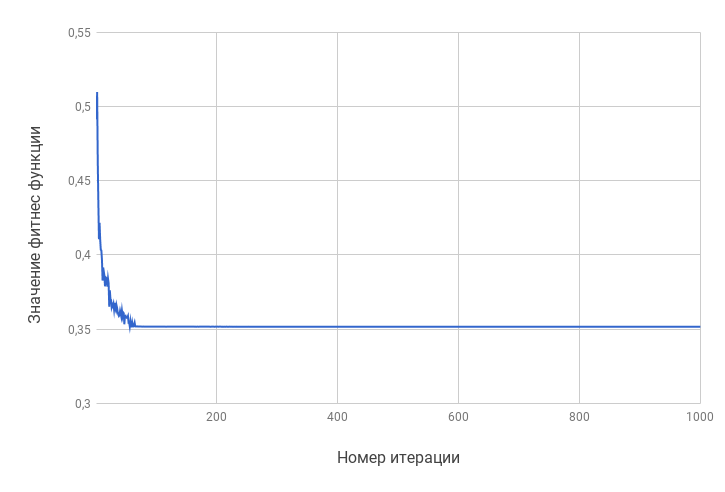
\includegraphics[scale=0.45]{gen_1.png}  
	\caption{Сходимость генетического алгоритма на тестовом наборе}
	\label{fig:gen_1}
\end{figure}

Как можно заметить, оптимальное решение находится еще на ранних итерациях, причем общее время выполнения не превышало пяти секунд.

Как можно видеть из гистограммы на рис. \ref{fig:gen_gist_fitness} сходимость подобного рода наблюдается на большинстве сгенерированных тестовых кейсов, однако в некоторых случаях оптимальное решение строится на гораздо более поздних итерациях. Данным фактом решено было пренебречь, так как гистограмма на рис. \ref{fig:gen_gist_probab} показывает, что оптимальность решения с точки зрения максимизации вероятности контакта злоумышленника с элементами обманной системы, а это является главной задачей в автоматизации процесса разворачивания обманной системы, достигалась на гораздо более ранних итерациях и всё последующее время алгоритм минимизирует количество задействованных ловушек.

\begin{figure}[ht]
\centering
	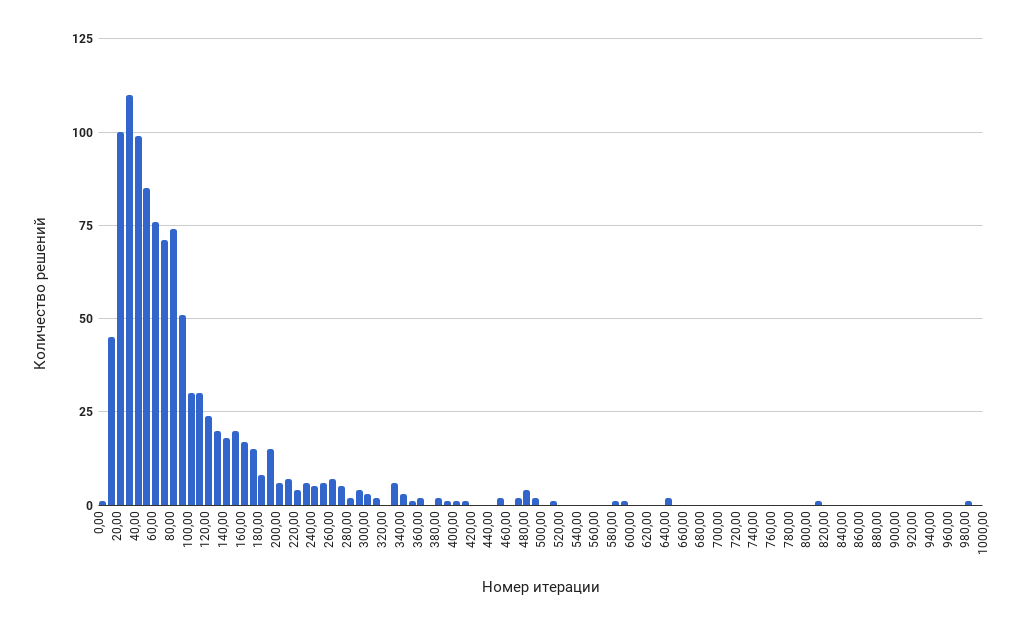
\includegraphics[scale=0.34]{gen_gist_fitness.png}  
	\caption{Гистограмма количества решений по номеру итерации, на котором алгоритм сходился по целевой функции}
	\label{fig:gen_gist_fitness}
\end{figure}

\begin{figure}[ht]
\centering
	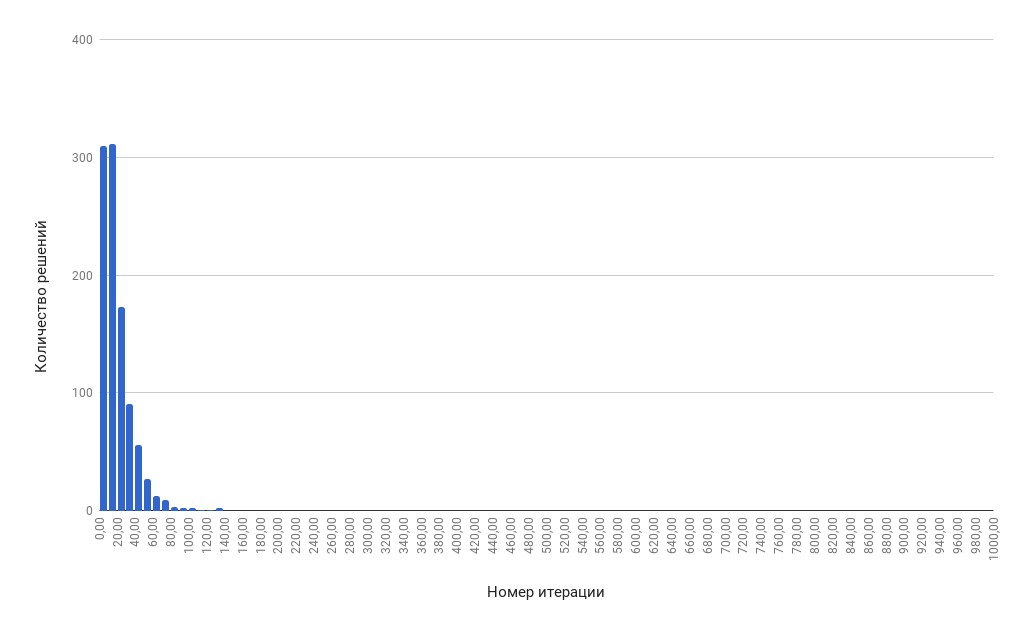
\includegraphics[scale=0.34]{gen_gist_probab.png}  
	\caption{Гистограмма количества решений по номеру итерации, на котором алгоритм сходился по вероятности $1 - P_{honey, min}$}
	\label{fig:gen_gist_probab}
\end{figure}